% Ch5.tex

\chapter{Long-term estimation of frog calling activity and species richness}
\label{cha:cha8Application}

In previous Chapters, various algorithms have been proposed for studying the frog call classification problem. In this chapter, the proposed algorithm will be applied to a three-months dataset for estimating frog calling activity and species richness. The dataset is constructed by sampling 10-second recordings every 10 minutes from continuous recordings over three months. Finally, there are 4170, 4908, and 1544 10-second recordings for \textit{Kiyomi dam}, \textit{Stony Creek dam} and \textit{BG Creek dam}, respectively, which are used for long-term acoustic monitoring. Here, the number of recordings of those three sites is different for the data loss in some days.


The architecture is shown in Figure~\ref{fig:Ch7_flowchart}. The system contains three parts: frog calling activity estimation, frog species richness estimation, and correlation analysis. Each part is discussed in detail in the following subsections.

\begin{figure}[htb!]
\centering
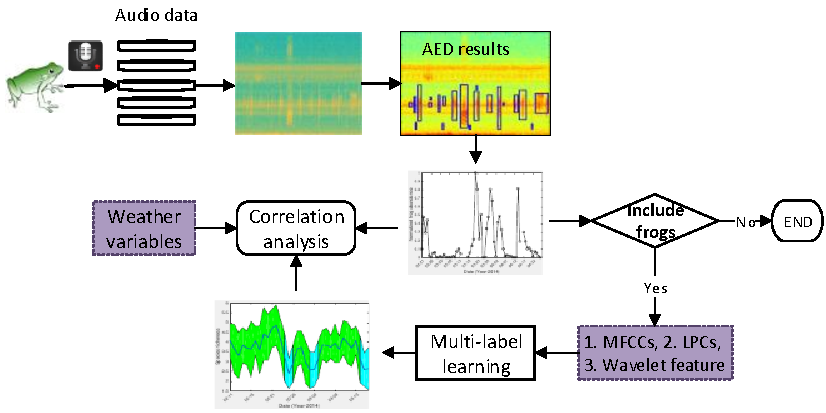
\includegraphics[width=\textwidth]{image/Ch7/flowchart.pdf}
\caption{Flowchart of a frog call classification system using AED and ML learning}
\label{fig:Ch7_flowchart}
\end{figure}




\section{Long-term monitoring of frog calling activity}

Frog calling activity is estimated through the detection of acoustic events in a spectrogram image. Here, the spectrogram is generated by applying STFT to each 10-second recording. The description of the AED method is shown in Chapter \ref{Ch5:AEDmethod}. Frog calling activity of each 10-second recording is estimated as 

\begin{equation}
F_{abun} = \sum_{n=1}^{N}\sum_{i=1}^{I}\sum_{j=1}^{J} A_{i,j}(n)^2
\end{equation}
Here, $A_{i,j}$ represents the decibel value of location $(i,j)$ within each acoustic event $n$ in the spectrogram, $i$ is the temporal index, $j$ is the frequency index, $I$ and $J$ are the height and width of each acoustic event.

\begin{figure}
        \centering       
        \begin{subfigure}[b]{0.35\textwidth}
                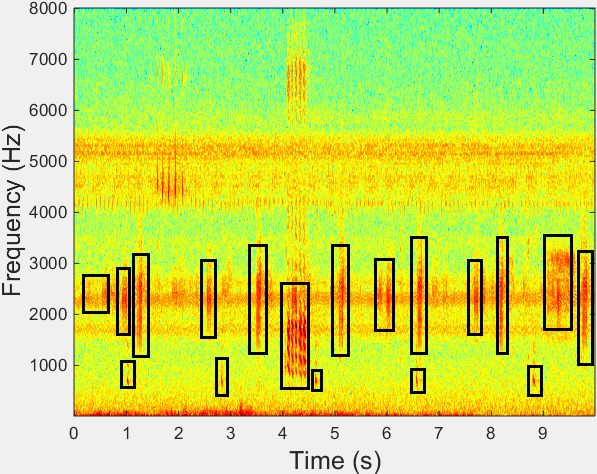
\includegraphics[width=\textwidth]{image/Ch7/spectrogram1-m.png}
                \caption{Baseline}
        \end{subfigure}%
 ~       
        \begin{subfigure}[b]{0.35\textwidth}
                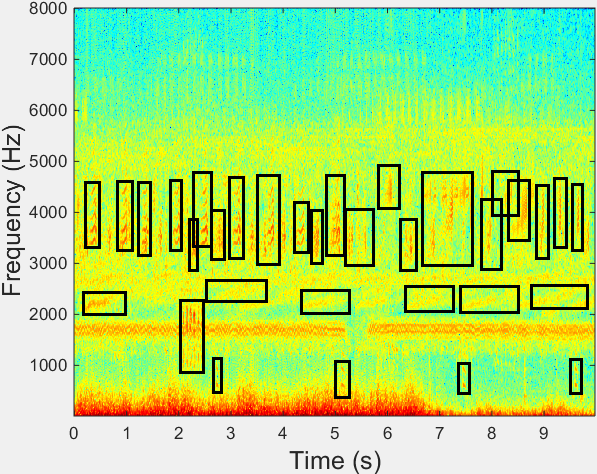
\includegraphics[width=\textwidth]{image/Ch7/spectrogram2-m.png}
                \caption{Baseline}
        \end{subfigure}%
        \\          
        \begin{subfigure}[b]{0.35\textwidth}
                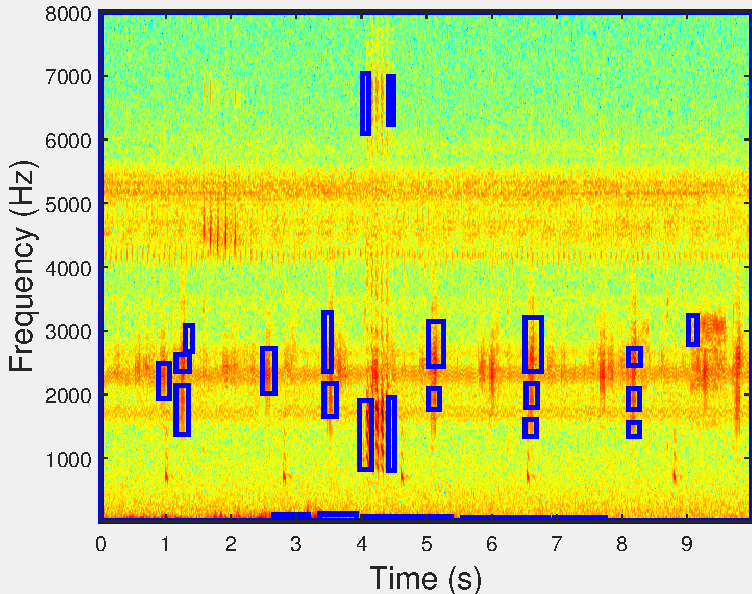
\includegraphics[width=\textwidth]{image/Ch7/AEDFodor.pdf}
                \caption{Method of \cite{fodor2013ninth}}
        \end{subfigure}%
                ~        
        \begin{subfigure}[b]{0.35\textwidth}
                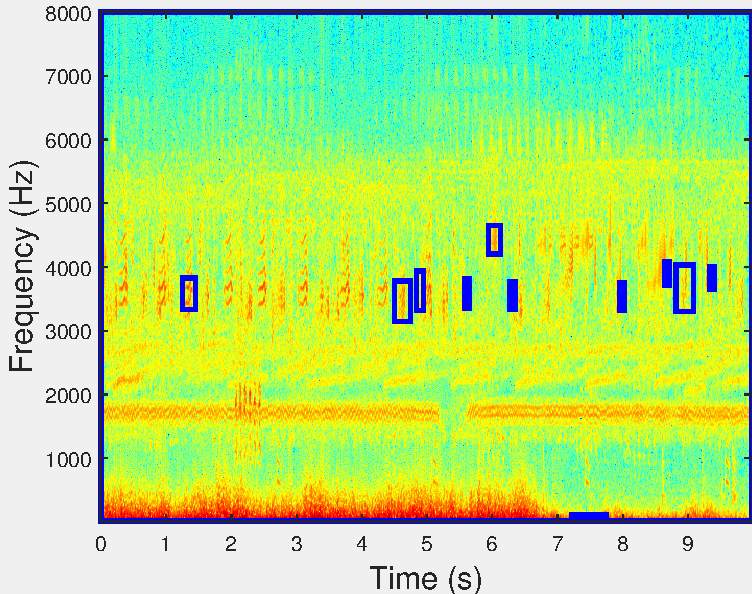
\includegraphics[width=\textwidth]{image/Ch7/AEDFodor_2.pdf}
                \caption{Method of \cite{fodor2013ninth}}
        \end{subfigure}
\\

               \begin{subfigure}[b]{0.35\textwidth}
                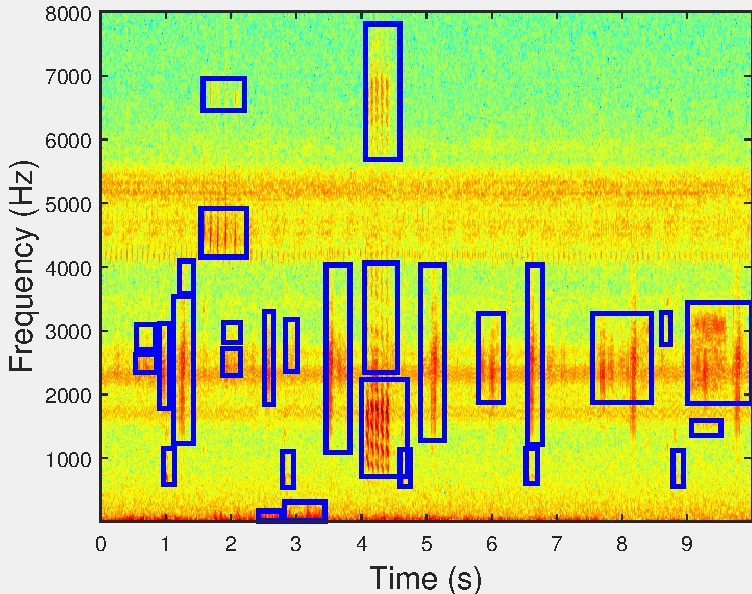
\includegraphics[width=\textwidth]{image/Ch7/AED_Michael.pdf}
                \caption{Method of \cite{Michael2011}}
        \end{subfigure}  
        ~  
                \begin{subfigure}[b]{0.35\textwidth}
                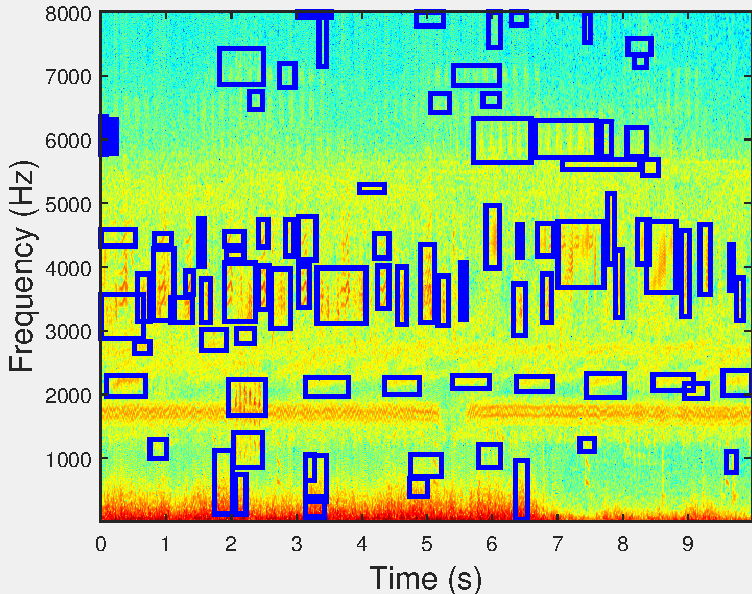
\includegraphics[width=\textwidth]{image/Ch7/AED_Michael_2.pdf}
                \caption{Method of \cite{Michael2011}}
        \end{subfigure}%              
\\         
                \begin{subfigure}[b]{0.35\textwidth}
       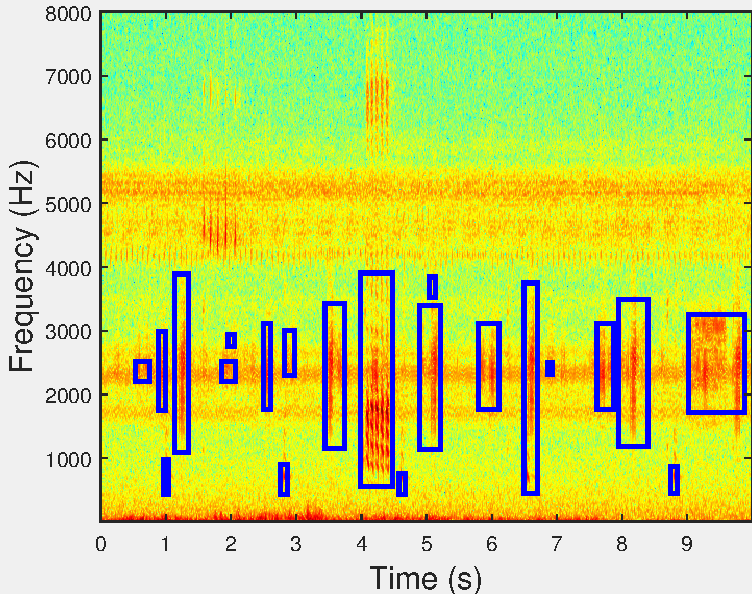
\includegraphics[width=\textwidth]{image/Ch7/AED_Jie.pdf}
                \caption{Proposed method}
        \end{subfigure}     
~
        \begin{subfigure}[b]{0.35\textwidth}
       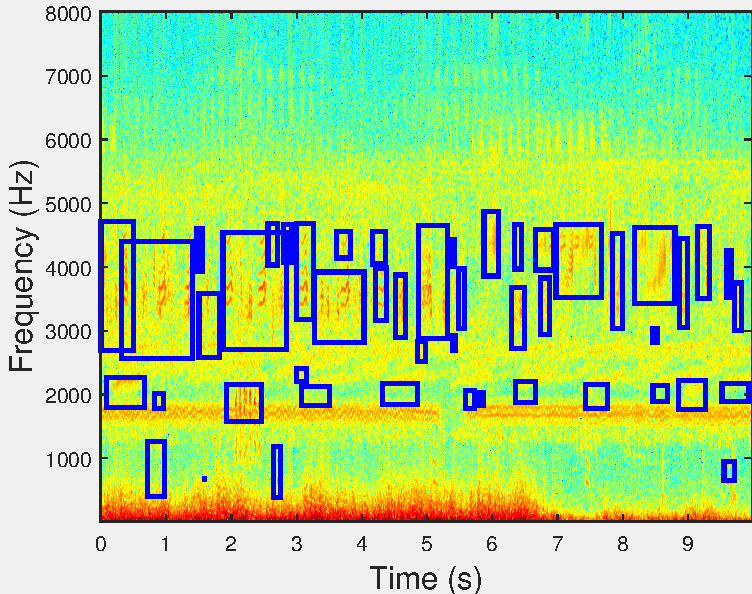
\includegraphics[width=\textwidth]{image/Ch7/AED_Jie_2.pdf}
                \caption{Proposed method}
        \end{subfigure}                
        \caption[AED for frog abundance monitoring using different methods]{AED for frog calling activity estimation using different methods. For each row, different methods are applied to the same recordings. The baseline of the detection results is shown in the first row; detected frog calls are drawn using a blue rectangle. For each column, different methods are used for the same recording.}        
        \label{fig:Ch7_AED}
\end{figure}




Figure~\ref{fig:frogAbundance} shows the frog calling activity results of three selected sites over the whole frog breeding season. It can be found that the frog calling activity of the same site changes a great deal over time. In the \textit{Kiyomi dam}, frog calling activity is relatively high from February 21 to February 25. However, frog calling activity is quite low in two periods, which are February 26 to March 11 and April 07 to April 12. The highest calling activity of this site is achieved on March 22. However, the highest calling activity for \textit{Stony Creek dam} and \textit{BG Creek dam} is obtained in February, which shows that frog calling activity of different sites often varies a lot for different environments. Recordings of 47 days of all three sites do not frog calls. In the subsequent analysis, only those recordings with frog calls are used for frog species richness estimation. 

\begin{figure}[htb!]
\centering
        \begin{subfigure}[b]{0.3\textwidth}
                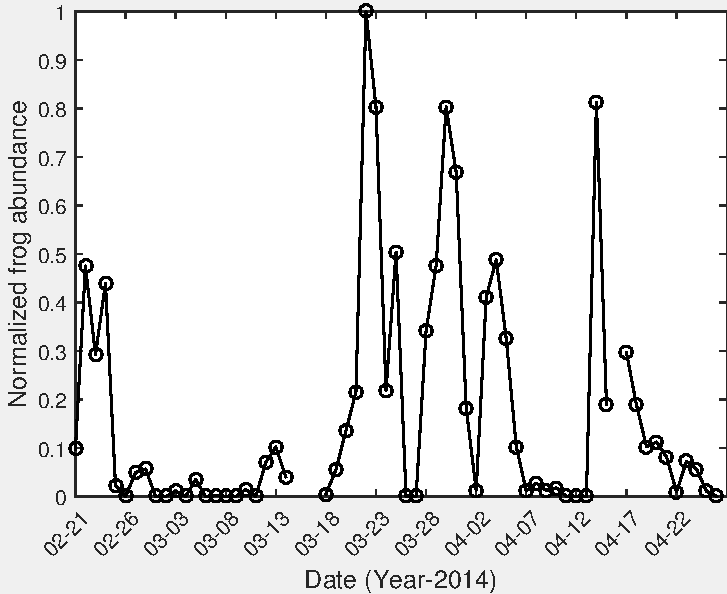
\includegraphics[width=\textwidth]{image/Ch7/abundance1075.pdf}
                \caption{\textit{Kiyomi dam}}
        \end{subfigure}
       ~
              \begin{subfigure}[b]{0.3\textwidth}
                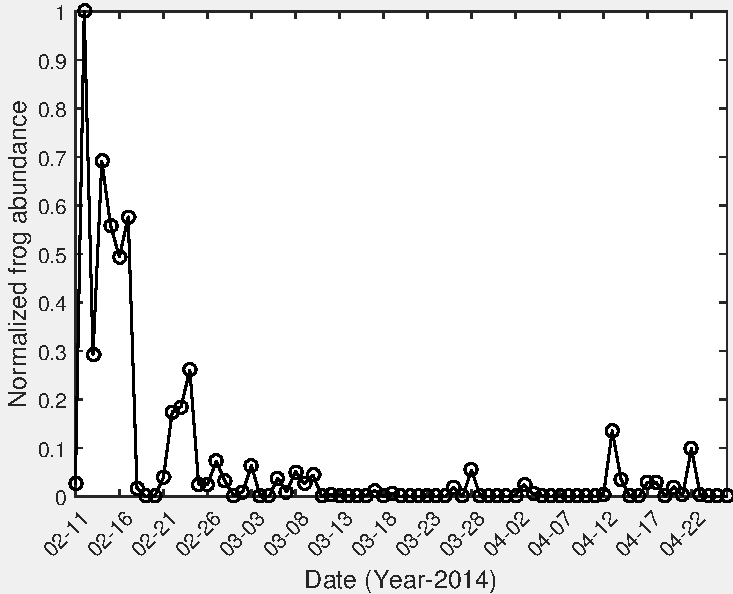
\includegraphics[width=\textwidth]{image/Ch7/abundance1078.pdf}     
                \caption{\textit{Stony creek dam}}           
        \end{subfigure} 
               ~
              \begin{subfigure}[b]{0.3\textwidth}
                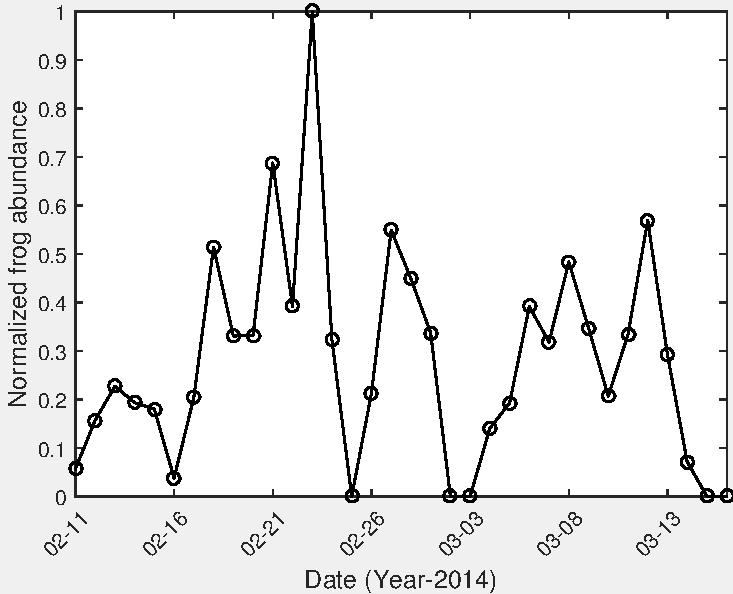
\includegraphics[width=\textwidth]{image/Ch7/abundance1079.pdf}     
                \caption{\textit{BG creek dam}}           
        \end{subfigure}       
\caption[Frog calling activity detection of different sites]{Frog calling activity estimation of different sites: \textit{Kiyomi dam}, \textit{Stony Creek dam} and \textit{BG Creek dam}. For \textit{Kiyomi dam}, three days do not record any acoustic data and then there is no value in those particular days. All the frog calling activity value is normalised to [0 1].}
        \label{fig:frogAbundance}
\end{figure}



\section{Long-term estimation of frog species richness}

Therefore, this combination is used for the testing data. 
Figure~\ref{fig:frogRichness} shows the frog species richness of the three selected sites. For all the three sites, the variation of species richness is not high, which shows that species richness of the same area is relatively stable. However, frog species richness of \textit{BG Creek dam} has a smaller variation over the time than \textit{Kiyomi dam} and \textit{Stony Creek dam}. The comparison of the species richness for the three sites is shown in Figure~\ref{fig:richnessSite}. In contrast to other sites, the species richness in \textit{BG Creek dam} is the highest. This might be that \textit{BG Creek dam} is closer to a river and farther away from the human community.
Frog species richness is estimated by predicting the species presence/absence of each sampled recording. 


The combination of multi-stage PWSCCs $+$ LPCs and the RAKEL1 method achieves the best performance. Therefore, this combination is used for the testing data. Figure~\ref{fig:frogRichness} shows the frog species richness of the three selected sites. For all the three sites, the variation of species richness is not high, which shows that species richness of the same area is relatively stable. However, frog species richness of \textit{BG Creek dam} has a smaller variation over the time than \textit{Kiyomi dam} and \textit{Stony Creek dam}. The comparison of the species richness for the three sites is shown in Figure~\ref{fig:richnessSite}. In contrast to other sites, the species richness in \textit{BG Creek dam} is the highest. This might be that \textit{BG Creek dam} is closer to a river and farther away from the human community.


\begin{figure}[htb!]
\centering
        \begin{subfigure}[b]{0.3\textwidth}
                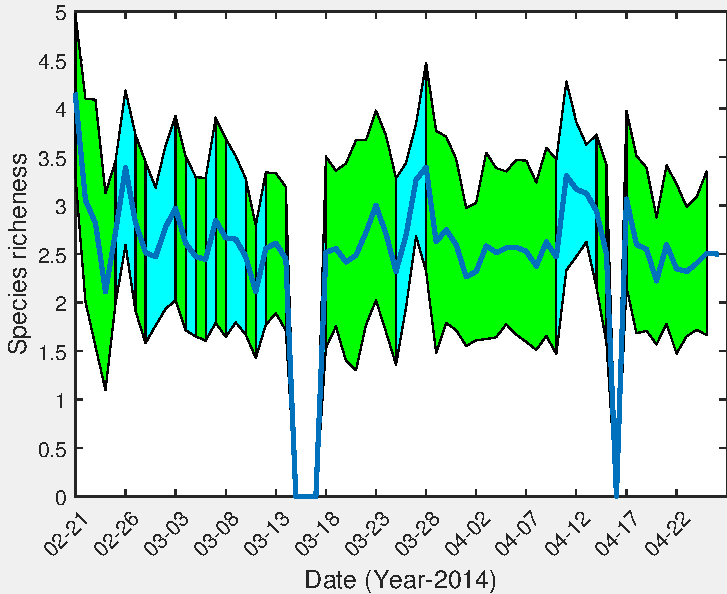
\includegraphics[width=\textwidth]{image/Ch7/richness1075.pdf}
                \caption{\textit{Kiyomi dam}}
        \end{subfigure}
       ~
              \begin{subfigure}[b]{0.3\textwidth}
                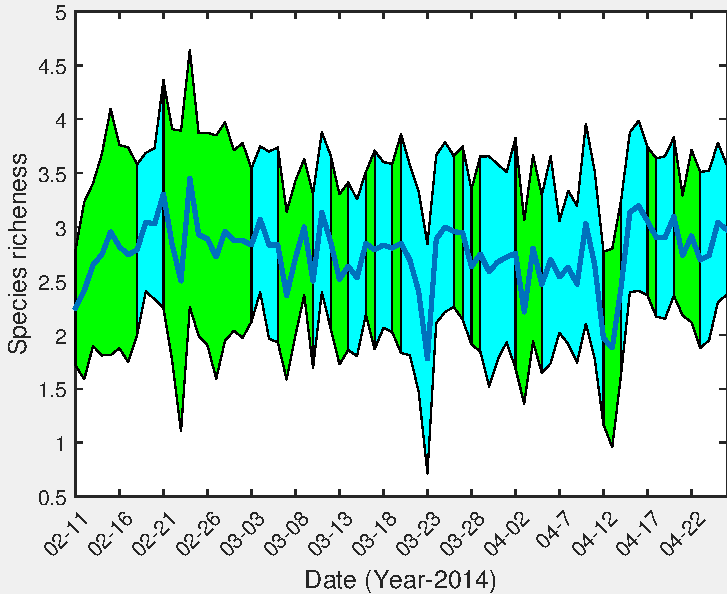
\includegraphics[width=\textwidth]{image/Ch7/richness1078.pdf}     
                \caption{\textit{Stony creek dam}}           
        \end{subfigure} 
        ~
              \begin{subfigure}[b]{0.3\textwidth}
                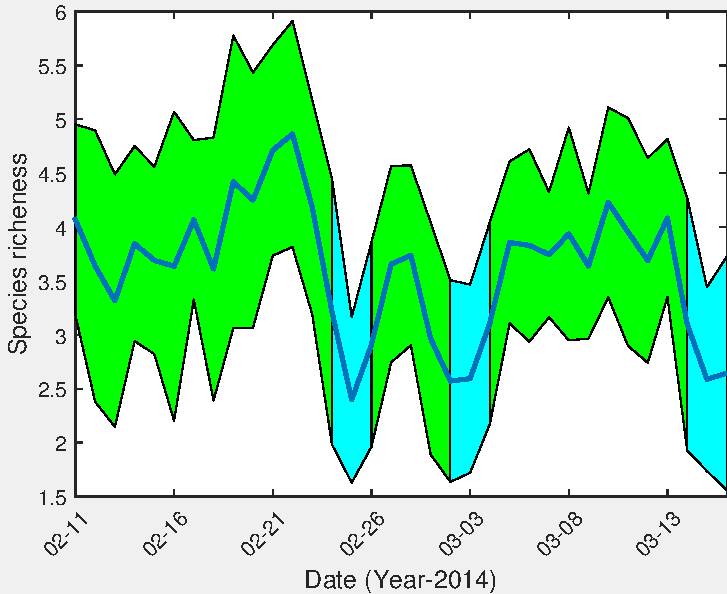
\includegraphics[width=\textwidth]{image/Ch7/richness1079.pdf}     
                \caption{\textit{BG creek dam}}           
        \end{subfigure}       
\caption[Frog species richness distribution of three selected sites]{Frog species richness distribution of three selected sites. Here green bar represents the species variation, blue bar means there is no frog calls, zero value denotes the data loss of those particular days.}
        \label{fig:frogRichness}
\end{figure}

\begin{figure}[htb!]
	\begin{centering}
	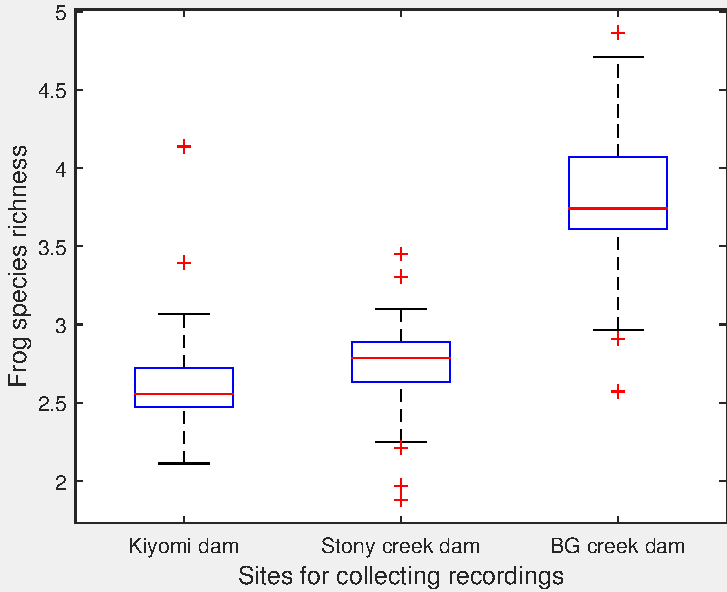
\includegraphics[width=0.5\textwidth]{image/Ch7/richnessSite.pdf}
	\caption{Averaged frog species richness of different sites.}
	\label{fig:richnessSite}
	\end{centering}
\end{figure}




\section{Statistical analysis}
Multiple regression analysis is used to explore the relationship between frog calling activity/species richness with weather variables (mean temperature and rainfall)\footnote[5] {http://www.bom.gov.au/?ref=hdr}. Both frog calling activity and species richness are found to be highly correlated with mean temperature (F=5.18, P\textless0.05 for calling activity, and F=10.7, P\textless0.01 for species richness). To calculate the correlation between rainfall and frog calling activity/species richness, we first set the rainfall vaule as the dummy variable. Then, the correlation between frog calling activity/species richness and rainfall value is also studied with multiple regression analysis (F=4.63, P\textless0.05 for calling activity, and F=4.64, P\textless0.05 for species richness). The statistical analysis results indicate that frogs tend to make calls in the warm and humid environment, which is in accordance to previous studies \citep{akmentins2015patterns, canavero2008calling}.


\section{Summary and limitations}






